\documentclass[twoside]{article}
\usepackage{graphicx}
\usepackage{polski}
\usepackage{fancyhdr}
\usepackage{lastpage}
\usepackage{epigraph}
\usepackage{listings}
\usepackage{soul}
\usepackage{color}
\usepackage{multirow}
\usepackage{subcaption}
\usepackage{fancyvrb}
\usepackage{hyperref}


\title{AiSD Ex. 4.2 (Pon.)}
\author{\hl{Mateusz Kamieniecki}}
\date{\today}

\lstset{
    numbers=left
}

\makeatletter

\begin{document}

\pagestyle{fancy}
\fancyhead{}
\fancyhead[L]{\@title}
\fancyhead[R]{\@author}
\fancyhead[C]{\@date}

\cfoot{\thepage\ / \pageref{LastPage}}


\newpage

\section{Wprowadzenie}

To, co dzisiaj jest nam niezbędne, pokażemy sobie na tablicy.

\section{Zadania}


\subsection{Zadanie 0}
Proszę (już tradycyjnie) uporządkować swoje repozytorium, aby organizacja projektów wyglądała jak poniżej. 
Oczywiście w tej strukturze mogą znajdować się również inne katalogi i pliki, ale proszę
dokładnie odwzorować przedstawiony porządek projektów.

\begin{verbatim}
.korzeń_repozytorium
+-- CW_0
|   +-- tak, jak poprzednio
|
+-- CW_1
|   +-- AiSD2026ZEx1
|       +-- pom.xml
|
+-- CW_2
|   +-- AiSD2026ZEx2
|       +-- pom.xml
|
+-- CW_3
|   +-- AiSD2026ZEx3
|       +-- pom.xml
+-- CW_4
    +-- AiSD2026ZEx4
        +-- pom.xml
\end{verbatim}

\newpage

\subsection{Zadanie 1}
Proszę zapoznać się z kodem źródłowym dołączonym do ćwiczenia.
Proszę zwrócić uwagę na metody interfejsu \verb|MapInterface| implementowane w klasie \verb|RbtMap|.
Klasa implementująca mapę (\verb|RbtMap|) wykorzystuje klasę \verb|RedBlackTree| dla generycznych typów danych klucza (\verb|K|) i wartości (\verb|V|).


\subsection{Zadanie 2}
Analizę i zrozumienia kodu należy potwierdzić implementując testy (w przeważającej liczbie powinny to być testy o charakterze testów jednostkowych).
Testy powinny weryfikować poprawność działania kodu zgodnie z ustaleniami podanymi w trakcie pierwszego spotkania dotyczącego bieżącego (czwartego) ćwiczenia.

Przy wykonaniu tego ćwiczenia proszę wspierać się analizą pokrycia kodu testami -- aby to ułatwić,
w konfiguracji projektu (\verb|pom.xml|) została dołączona wtyczka z biblioteką \textbf{JaCoCo}.

Chcąc sprawdzić aktualne pokrycie kodu testami należy wykonać fazę \textbf{package} cyklu życia projektu maven-owego:
\begin{itemize}
    \item z poziomu NetBeans-a: klikamy prawy przycisk myszy (PPM) na projekcie 
    \verb|->| \textbf{Run Maven}
    \verb|->| \textbf{Goals} lub \textbf{Other Goals} zależnie od wersji IDE
    \verb|->| w polu oznaczonym \textbf{Goals} wpisujemy: \textbf{package};
    \item lub z wiersza poleceń: \verb|mvn clean package|.
\end{itemize}

Po udanym zakończeniu fazy pakowania w głównym katalogu projektu powstanie katalog \textbf{target},
a w nim powinny być: \textbf{site} \verb|->| \textbf{jacoco} \verb|->| \textbf{index.html}.
W ulubionej (lub tej dostępnej pod ręką) przeglądarce otwieramy \textbf{index.html} i analizujemy
wynik. Staramy się, aby procentowe pokrycie kodu testami było jak największe.


\subsection{Zadanie 3}
W pakiecie testów (\verb|test/|\verb|java/|\verb|pl/|\verb|edu/|\verb|pw/|\verb|ee/|\verb|aisd2026zex4/|\verb|performance|) proszę stworzyć klasę \verb|DataGenerator| z metodami
generującymi dane (o rozmiarze \verb|size|) w trzech porządkach (losowym, rosnącym, malejącym):
\begin{itemize}
    \item \verb|public String[] generateRandData(int size)|;
    \item \verb|public String[] generateAscData(int size)|;
    \item \verb|public String[] generateDescData(int size)|.
\end{itemize}


\subsection{Zadanie 4}
W klasie \verb|RedBlackTree| jest prywatna metoda usuwająca ,,najmniejszy'' klucz (wraz z wartością).
Należy uzupełnić jej implementację na podstawie własnej intuicji lub korzystając z poniższego opisu dla usuwania klucza ,,największego'' (a nie ,,najmniejszego''\textbf{!}).

\begin{enumerate}
    \addtocounter{enumi}{-1}
    \item Zabezpieczamy się przed usunięciem "czegoś" z pustego drzewa.
    \item Sprawdzamy, czy lewy potomek naszego węzła jest czerwony.
        \begin{itemize}
            \item FALSE: nic nie zmieniamy.
            \item TRUE: wykonujemy rotację w prawo na naszym węźle i w ten sposób naszym nowym
                węzłem staje się wynik rotacji.
        \end{itemize}
    \item Sprawdzamy, czy przypadkiem nie dotarliśmy już do węzła, który nie ma prawego potomka.
        \begin{itemize}
            \item FALSE: nic nie zmieniamy.
            \item TRUE: zwracamy null jako potwierdzenie (w wywołaniu rekurencyjnym zwrócony
                ,,null''  zostanie zapisany jako prawy potomek rodzica, który przed chwilą miał
                największego (w całym drzewie) prawego potomka).
        \end{itemize}
    \item Sprawdzamy, czy prawy potomek naszego węzła NIE jest czerwony (co nie oznacza, że jest
        czarny) oraz czy lewy potomek prawego potomka naszego węzła NIE jest czerwony (co też nie
        oznacza, że jest czarny).
        \begin{itemize}
            \item FALSE: nic nie zmieniamy.
            \item TRUE: (ani prawy, ani lewy od prawego nie jest czerwony) robimy zamianę kolorów.
            \item TRUE.A. Sprawdzamy, czy nasz węzeł ma lewego potomka i czy lewy potomek tego
                lewego potomka jest czerwony.
                \begin{itemize}
                    \item TRUE.A.FALSE: nic nie robimy
                    \item TRUE.A.TRUE: wykonujemy rotację w prawo na naszym węźle i w ten sposób
                        naszym nowym węzłem staje się wynik rotacji. Następnie jeszcze raz
                        wykonujemy zamianę kolorów.
                \end{itemize}
        \end{itemize}
    \item Robimy wywołanie rekurencyjne naszej metody usuwającej i jako parametr wywołania
        przekazujemy prawego potomka od naszego węzła. A wynik rekurencyjnego wywołania 
        przypisujemy jako prawy potomek naszego węzła. (W ten sposób nawiązujemy do punkt 2.)
    \item Wykonujemy naprawę naszego drzewa (tylko w tym węźle, w którym aktualnie jesteśmy).
        \begin{enumerate}
            \item Wykonujemy rotację w lewo (jeśli prawy potomek jest czerwony).
            \item Wykonujemy rotację w prawo (jeśli obydwa kolejne lewe potomki są czerwone).
            \item Wykonujemy zamianę kolorów (jeśli prawy potomek i lewy potomek są czerwone).
        \end{enumerate}
    \item Jako wynik działania metody rekurencyjnej zwracamy wynikowy węzeł po operacjach
        z punktu 5.
    
\end{enumerate}

\newpage

\subsection{Zadanie 5}
Proszę, wykorzystując suplement z kodem źródłowym (załącznik z ISOD-a), przygotować wykres 
(rys. \ref{fig:rbt_rand_height}) pokazujący, jak zmienia się wysokość drzewa czerwono-czarnego 
(jednostronnie, lewostronnie czerwonego), gdy wstawiamy do niego klucze w porządku losowym.
Proszę, odwołując się do teorii i swojej wiedzy, ustalić, czy wynikowy wykres jest ,,sensowny''.
Proszę odpowiedzieć, jak wyglądałby wynikowy wykres, gdyby wstawiane dane (klucze) były wstawiane
w~porządku rosnącym. A jak wyglądałyby dane wstawiane w porządku malejącym?

\begin{figure}[h]
    \centering
    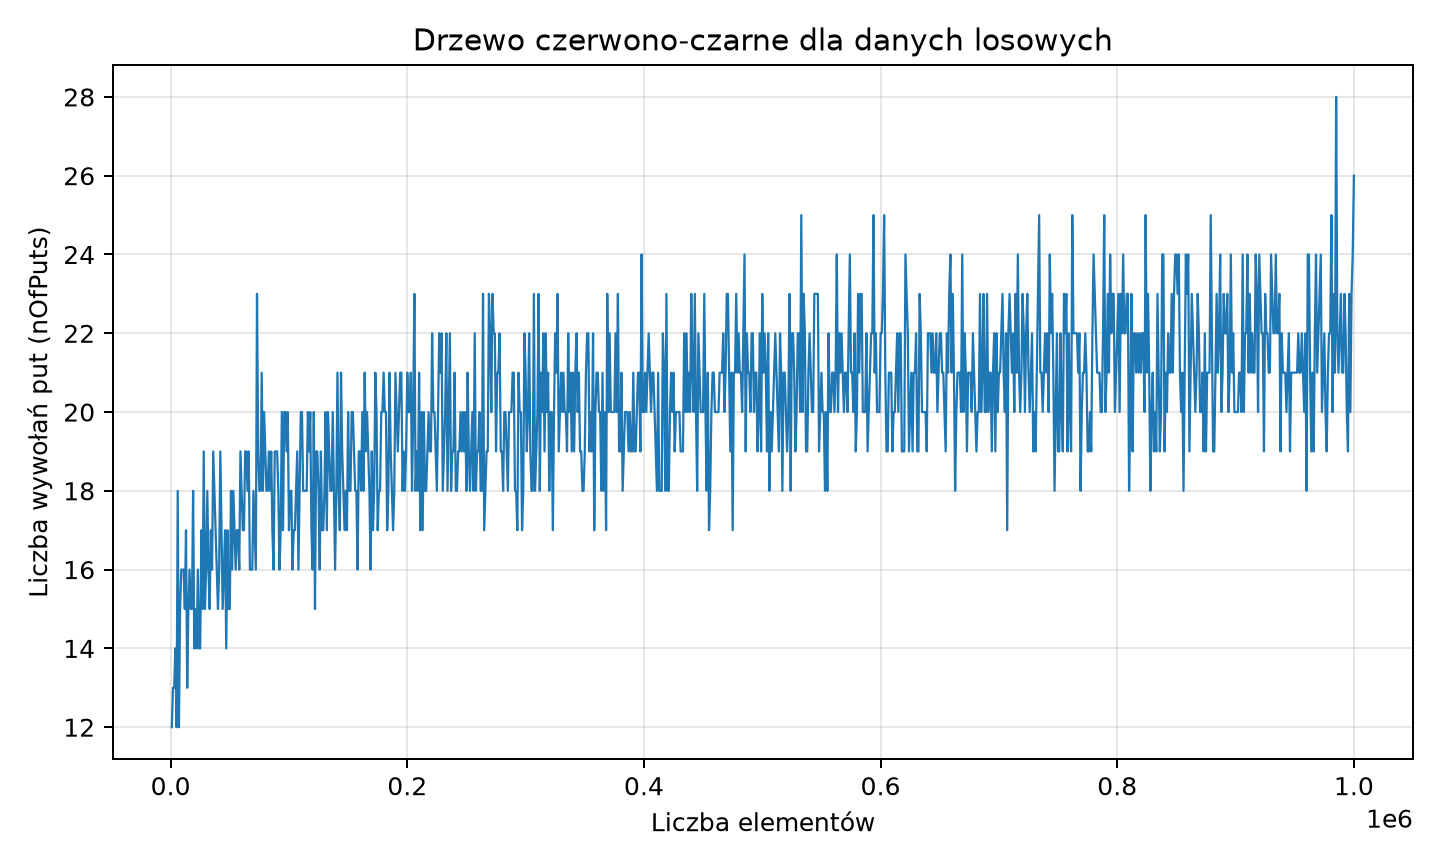
\includegraphics[width=\textwidth]{images/rbt_rand_data_tree_height.png}
    \caption{Liczba wywołań rekurencyjnej metody \texttt{put} podczas wstawiania danych losowych do drzewa czerwono-czarnego.}
    \label{fig:rbt_rand_height}
\end{figure}

\noindent \textbf{Wnioski:}

Wykres wygląda sensownie: wraz ze wzrostem liczby elementów liczba wywołań
\verb|put| ogólnie rośnie, ale lokalnie może się zmniejszać. Wynika to z losowej
kolejności kluczy i różnej głębokości, na której trafia kolejny element.

Dzięki rotacjom i zmianom kolorów drzewo pozostaje zrównoważone, więc wzrost
jest zbliżony do logarytmicznego. Dla danych rosnących i malejących oczekiwany
byłby podobny wynik. \verb|nOfPuts| nie oznacza jednak dokładnej wysokości
drzewa, lecz liczbę wywołań \verb|put| dla ostatnio wstawianych danych.

\newpage

\subsection{Zadanie 6}
Odwołując się do teorii (z wykładu lub materiałów uzupełniających: ,,Wprowadzenie do algorytmów'',
Cormen, Leiserson, Rivest, Stein), proszę podać przykład (sekwencję elementów wkładanych do (lub 
usuwanych z) początkowo pustego drzewa czerwono-czarnego) prowadzący do sytuacji wystąpienia węzła
,,podwójnie czarnego'' w klasycznym RBT.
Proszę krótko wyjaśnić, dlaczego dany przykład doprowadzi do takiej sytuacji.

\noindent \textbf{Przykład:}

Do początkowo pustego klasycznego drzewa czerwono-czarnego wstawiamy kolejno
klucze \(2, 1, 3\). Po zakończeniu wstawiania otrzymujemy:

\begin{verbatim}
        2(B)
       /   \
    1(B)   3(B)
\end{verbatim}

Następnie usuwamy klucz \(1\). Jest to czarny liść, więc po jego usunięciu
w jego miejscu pozostaje czarny węzeł wartowniczy \(\mathrm{NIL}\). Usunięcie
czarnego węzła zmniejsza liczbę czarnych węzłów na ścieżce z korzenia, dlatego
otrzymany węzeł \(\mathrm{NIL}\) traktujemy jako ,,podwójnie czarny''. Dodatkowa
Czerń nie jest rzeczywistym kolorem zapamiętanym w węźle, lecz oznacza
konieczność wykonania procedury naprawiającej własność czarnych wysokości drzewa.

\newpage

\subsection{Zadanie 7}

Załóżmy, że do niepustego drzewa RB (jednostronnie, lewostronnie czerwonego) wstawiliśmy węzeł "x", a następnie (od razu po wstawieniu) usunęliśmy ten węzeł. 
Czy drzewo, które powstało po usunięciu "x" jest takie samo jak drzewo przed wstawieniem "x"? 

Proszę podać uzasadnienie wraz z narysowaniem (właściwych z punktu widzenia odpowiedzi) sekwencji 
tworzenia drzew. Proszę oszczędnie wykorzystywać miejsce -- odpowiedź powinna zmieścić się na 
jednej stronie. 

\noindent \textbf{Miejsce na odpowiedź i rysunki:} \hl{TODO ------------------}.

\newpage

\subsection{Zadanie 8}
Proszę zmodyfikować metodę testową \verb|countTreeHeightDependingOnDataSize| w taki sposób, aby
po zakończeniu pętli \verb|while| była wyświetlana (wcześniej trzeba policzyć) liczba czerwonych węzłów wynikowego drzewa -- proszę uzupełnić tabelę \ref{Tab:red-nodes-counter} zebranymi wynikami.
Proszę skomentować uzyskane wyniki.

Być może, aby zrealizować to zadanie, trzeba będzie zmodyfikować kod w~klasach: \verb|RbtMap|,
\verb|RedBlackTree|, aby dostać się do korzenia drzewa. 
A czy da się to osiągnąć bez modyfikowania kodu?
Wcześniej korzystaliśmy z mechanizmu refleksji.
Czy tutaj również można go zastosować?
Jeśli się Państwu uda, to proszę się tym pochwalić w dodatkowym komentarzu pod tabelą.

\begin{table}[h!]
\begin{tabular}{|l|l|}
\hline
Rodzaj danych & Liczba czerwonych wezłów \\ \hline
Losowe        &                          \\ \hline
Rosnące       &                          \\ \hline
Malejące      &                          \\ \hline
\end{tabular}
\caption{}
\label{Tab:red-nodes-counter}
\end{table}

\noindent \textbf{Miejsce na komentarz do tabeli} \hl{TODO ------------------}.

\newpage

\subsection{Zadanie 9}
Proszę na rys. \ref{fig:jacoco_result} zamieścić wynik (zrzut ekranu z głównej strony wyników JaCoCo) pokrycia kodu testami z najnowszej (ostatniej, uzupełnionej) wersji kodu.

\begin{figure}[h]
    \centering
    \includegraphics{example-image-a}
    \caption{Wynik pokrycia kodu testami (JaCoCo).}
    \label{fig:jacoco_result}
\end{figure}

\section{Na zakończenie}
To już prawie koniec, ale tak jak poprzednio nie wolno nam zapomnieć, że:
\begin{itemize}
    \item wszystkie zmiany (cały kod źródłowy) muszą trafić do repozytorium.
    A~ostatnią zmianę (\textit{commit}) w repozytorium zdalnym należy oznaczyć tagiem
    \textbf{ze znacznikiem czasowym} \textbf{CW\_4\_FINAL};
    \item końcową wersję tego dokumentu (PDF) należy umieścić w ISOD-zie;
    \item \textbf{uwaga:} niewykonanie któregoś z powyższych dwóch kroków będzie oznaczało niewykonanie ćwiczenia, co jest równoznaczne z brakiem zaliczenia.
\end{itemize}

\end{document}
